\documentclass[12pt]{article}
\usepackage[T2A,T1]{fontenc}
\usepackage[english,russian]{babel}
\usepackage{graphicx}
\usepackage{tikz-qtree}

    \title{\textbf{Д/З ЕГЭ Информатика}}
    \author{Юрченко Александр 11 "А"}
    \date{}
    
    \addtolength{\topmargin}{-2cm}
    \addtolength{\textheight}{2cm}
\begin{document}

\maketitle
\thispagestyle{empty}
\section*{№1}
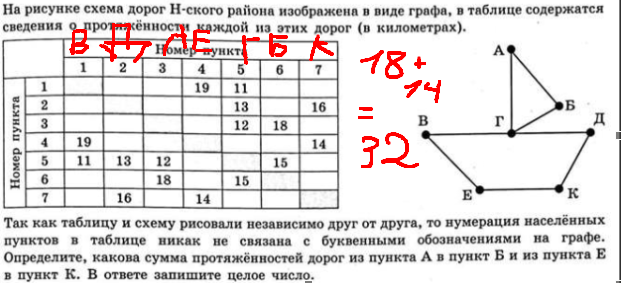
\includegraphics[scale=0.5]{first.png}
Ответ: 32

\section*{№2}
Код:
\begin{verbatim}
def f(x,y,z,w):
    return x and (y<=z) and ((not y) <= ((not z)==w))

for x in range(2):
    for y in range(2):
        for z in range(2):
            for w in range(2):
                if f(x,y,z,w)==1:
                    print(x,y,z,w,"|",f(x,y,z,w))
\end{verbatim}
Изначальные данные
\begin{verbatim}
\end{verbatim}
\pagebreak
Резултирующие данные
\begin{verbatim}
\end{verbatim}
Ответ: xzyw


\section*{№3}
\begin{verbatim}
\end{verbatim}
Ответ:

\end{document}

